\documentclass[]{report}
\usepackage{ucs}
\usepackage[latin1]{inputenc}
\usepackage[english]{babel}
\usepackage{amsmath}
\usepackage{marvosym}
%\usepackage{hyperref}
\usepackage[colorlinks=true,
            linkcolor=black,
            urlcolor=blue,
            citecolor=black]{hyperref}
\usepackage{breakurl}
\usepackage{fancyhdr}
\usepackage{graphicx}
\usepackage{float}
\usepackage[margin=2.7cm]{geometry}
\pagestyle{fancy}
\usepackage{subfig}
\usepackage{color, colortbl}
\usepackage{extraplaceins}
\usepackage{listings}

\lstset{
basicstyle=\sffamily\small,        % the size of the fonts that are used for the code
showspaces=false,                   % show spaces adding particular underscores
showstringspaces=false,           % underline spaces within strings
showtabs=false,                   % show tabs within strings adding particular underscores
frame=single,                      % adds a frame around the code
tabsize=2,                        % sets default tabsize to 2 spaces
captionpos=t,                     % sets the caption-position to bottom
breaklines=true,                  % sets automatic line breaking
breakatwhitespace=false,           % sets if automatic breaks should only happen at whitespace
escapeinside={\%*}{*)},            % if you want to add a comment within your code
morekeywords={*,...}               % if you want to add more keywords to the set
}   


\fancyhead{}

\lhead{Advanced Natural Language Processing}
\chead{}
\rhead{}
\lfoot{
\includegraphics[scale=0.2]{img/upc}}
\cfoot{\thepage}

% Title Page
\title{Demonym gazetteer}
\date{29\textsuperscript{th}, May 2014}
\author{Alex Pardo and David Sanchez}


\begin{document}
\maketitle

\tableofcontents

\newpage

\section{Introduction}

Demonym or gentilic, is a term for the residents of a locality. 
How to generate the demonym from a country or city name is not an easy task, and in order to automatize this process we are proposing a system which which will be capable to do it. 
The next document will show the description of the problem, our system approach, the evaluation and the discussions of the results. Finally, we will explain some possible improvements in our work as a future work.

\section{Attached files}

The structure of the project is separated into two files: demonym.py and functions.py.
\begin{itemize}
\item \textbf{Demonym.py}: Contains the main code which it calls all the methods from function.py. The methods are the following:

\item \textbf{Functions.py}:  Contains all the methods of the system.
\begin{itemize}
\item  \textit{demonyms\_downloadDemonymsWP:} Extracts pairs of country-demonym from wp.
\item  \textit{demonyms\_showHistogram:} Parses the rule file and extracts adding and replacing rules. Finally, shows the histogram.
\item  \textit{demonyms\_parseFile:} Parses the demonym file.
\item  \textit{demonyms\_generateRules:} Extracts the rule for a given pair country, demonym.
\item  \textit{demonyms\_parseCitiesAndCountries:} Download a list of cities  and a list of countries from Wikipedia.
\item  \textit{demonyms\_generateDemonym:} Generates all the possible demonyms from a given place.
\item  \textit{demonyms\_matchCandidates:} Finds the given demonym candidates in the WP of the given place.
\item  \textit{demonyms\_findWholeWord:} Finds a whole word.
\item  \textit{demonyms\_findDemonyms:} Extracts the rules from the files, reads the sample (i.e places) and perfoms the matching.
\item  \textit{demonyms\_guessEncoding:} Detects coding and transforms to Unicode
\end{itemize}
\end{itemize}

Finally, data files need for the system are the \textbf{cities.csv}, \textbf{countries.csv}, and \textbf{demonyms.csv}.
%Identifiers of the attached files (classes, functions and script .py files and data files when needed)

\section{Description of the problem}

As the document mentions in the introduction, the generation of the demonym from a location like country or city is not an easy task. There exist a lot of possible rules and different cases. 
\vspace{0.5cm}
Some examples of this process are:
\begin{itemize}
\item Africa -- African
\item Croatia -- Croatian (also "Croat")
\item North / South Korea -- North / South Korean
\item Hanoi (Vietnam) -- Hanoian
\item Iran -- Iranian (also "Irani" or "Persian")
\item Florence -- Florentine (also Latin "Florentia")
\item Ann Arbor -- Ann Arborite
\item Israel -- Israelite (also "Israeli")
\item Netherlands -- Netherlander
\end{itemize}

As the examples above show, some demonyms are simple a process in which is needed to add or replace ending letters in the original country or city. However, irregular cases are the ones that complicate the task of extracting general rules since are special cases and require a specific norms. We have to assume that we are not going to be able to generate those demonyms that are more difficult because are irregular forms or just because there are few cases.


\newpage
\section{Approach}


Our system follows the general flow in this type of systems which it is based on two phases: training and test (Figure \ref{Main architecture of our system.}). 

In the training phase the system obtains a database of examples (in this case from Wikipedia) of country demonyms\footnote{See \href{Wikipedia Demonym page}{http://en.wikipedia.org/wiki/Demonym}} and extracts rules from them.
In order to remove special cases, a threshold is used in order to filter out those rules which appear less than 3 times.

We have defined two types of rules:
\begin{itemize}
\item Adding rules: in which only a suffix is added to the location.
\item Substitution rules: in which some letters of the location are substituted by a suffix.
\end{itemize}

An example of this two types of rules in the pair Africa - African will be:
\begin{itemize}
\item "a" - "an"
\item " " - "n"
\end{itemize}

Once all the rules are generated and stored, the system extracts two test datasets also from Wikipedia; one is a list of cities in the world and the other a list of countries. Although the source is completely different from the one used in the training phase, some of the locations might be repeated but since the rules do not take into account the location but only the ending of the words it should not influence in the results.

When we have our two test sets, for every location we generate all the demonyms applying all the possible rules and find them in the Wikipedia page of the country/city. Notice that in almost all the city/country pages the demonym appears several times. In some cases, it never appears. Since we are not able to distinguish this two cases, in order to simplify the problem we are going to assume that all the pages have the demonym in the text and it is always correct. 


This approach is the most direct and the commonly followed in every machine learning problem. Some decisions were taken in order to simplify the problem and are taken into account in the evaluation made. There are several ways to tackle this problem (e.g. using more complex suffixation techniques) but it makes more sense to begin with the simplest approach and if the results are not as good as expected, increase the complexity of the model. Several times, using a more complex model difficult the task of learning and the results are even worst than with a simpler one.

%Architecture of the system
\begin{figure}[htb!]
\centering
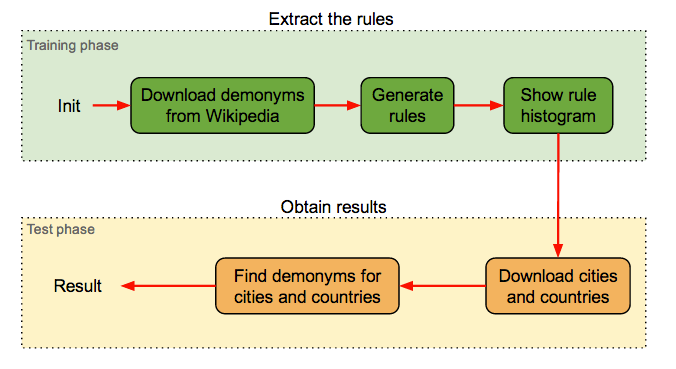
\includegraphics[scale=0.5]{img/architecture}
\caption{Main architecture of our system.}
\label{Main architecture of our system.}
\end{figure}

%Histogram figure
\begin{figure}[htb!]
\centering
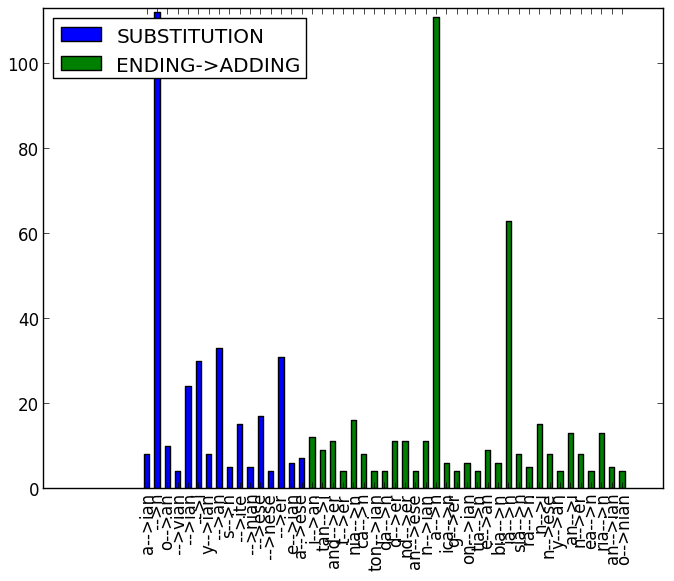
\includegraphics[scale=0.6]{img/rules}
\caption{Histogram of the rules.}
\label{Histogram of the rules.}
\end{figure}



%IMPORTANT:
%A description of the approach used for solving the problem. It is
%important to argument why this approach has been followed against the
%possible alternatives.

\section{Evaluation}

As it has been explained in the previous section, we generate all the demonyms using the possible rules and try to find them in the Wikipedia page of the city/country. For simplicity we assume that the correct demonym is always present in the Wikipedia page and that there are no mistakes.

In order to evaluate the algorithm, we simply count the number of demonyms found and the total number of locations we have and compute an Accuracy measure (here we do not have negative results):
$$
AC = \frac{true\_positive}{total\_population}
$$

As we are assuming that all the examples have a positive match in the text, in this case the Precision measure will have the same value.

\section{Results}

After performing the tests, we have the following results (See \textit{Execution results appendix} for the complete output):
\begin{itemize}
\item Cities: 89 matchings over 1751 cities, 5.08\% of accuracy.
\item Countries: 55 matchings over 89 countries, 61.8\% of accuracy.
\end{itemize}



\section{Discussion}

After looking at the results, one can see that the obtained accuracy in countries is acceptable but the value for cities is really low.

There are three considerations that have to be taken into account, first of all the system is trained only using countries and the obtained rules can be restricted to this types of locations; second, there are several cities with a really short page in Wikipedia (e.g. small cities of Africa or Asia) where the demonym is not appearing; and third, there are several cases of irregular forms, deriving for example from latin forms (Tarragona, Tarraconense).

All this factors are decreasing the accuracy of the system and have to be taken into account in the evaluation.


\section{Future work}

As a results shows, the accuracy of the cities is very lower and one improvement could try to obtain better results with the cities. The system had trained using only countries and maybe we could add other trained version of the system using only cities. The behaviour of the transformations needed to convert the country or city into the demonym sometimes differ if you are using cities and countries. For this reason we could include one system trained with the countries and other with the cities. 
\\\\
Other important improvement will be increase the complexity of the rules models because our rules models are very simple now. Also, the analyse of the word could be deeper using lexemes and so on.
\\\\
Finally, we could try to generalize the rules in order to reduce the rules which they are very specific.

\section*{Appendix}
\subsection*{Execution results}

Here we have the output of an execution of the whole system:

\lstinputlisting[breaklines]{experiment.res}


\end{document}          
